\chapter{Механика}
\section{Объекты классической механики}
\begin{itemize}
    \item \define \textbf{\textit{Материальная точка}} - это тело, размерами которого можно пренебречь по сравнению с его пространственным перемещением.
    \item \define \textbf{\textit{Система материальных точек} }- это множество материальных точек, положение и движение каждой из которых зависит от положения и движения остальных точек множества.
    \item \define \textbf{\textit{Абсолютно твердое тело}} - тело, деформациями которого можно пренебречь по сравнению с его пространственным перемещением.
    \item \define \textbf{\textit{Сплошная среда}} - всюду плотное множество материальных точек (жидкость, газы, деформируемые твердые тела).
\end{itemize}

\vspace{5px}

\underline{\textbf{Три постулата классической физики}}
\begin{enumerate}
    \item Считается возможным одновременное измерение с любой точностью всех физических величин, описывающих данное тело.
    \item Во всех системах отсчета промежуток времени между двумя событиями считается одинаковым.
    \item Во всех системах отсчета расстояние между двумя телами в данный момент времени считается одинаковым.
\end{enumerate}

\underline{\textbf{Разделы классической механики}}

\vspace{5px}

\define \textbf{\textit{Кинематика}} --- раздел механики, который изучает перемещение тел друг относительно друга без учета причин, вызывающих это движение.

\vspace{5px}

\define \textbf{\textit{Статика}} --- раздел механики, который изучает условия равновесие тел.

\vspace{5px}

\define \textbf{\textit{Динамика}} --- раздел механики, который изучает механическое движение тел с учетом причин, вызывающих это движение.

\vspace{3px}

\section{Кинематика}
\subsection{Кинематика материальной точки}
\define \textbf{\textit{Траектория}}--- линия, по которой движется материальная точка.

\vspace{5px}

\define \textbf{\textit{Радиус-вектор}} --- вектор, соединяющий тело отсчета с материальной точкой. Обозначается $\vec r$.

\vspace{5px}

\define \textbf{\textit{Вектор перемещения (или перемещение)}} --- вектор, соединяющий начальное положение материальной точки с ее текущим положением. Обозначается $\Delta \vec r$.

\vspace{5px}

\define \textbf{\textit{Путь}} - полное расстояние, пройденное точкой по траектории. Величина пути всегда неотрицательна. Обозначается s.

\vspace{5px}

\textbf{Способы задания движения точки в пространстве}
\begin{enumerate}
    \item \underline{Векторный} : задаются тело отсчета и радиус-вектор точки в зависимости от времени $\vec r(t)$.
    \item \underline{Координатный:} задаются точка отсчета, система координат, координаты точки в зависимости от времени x(t), y(t), z(t).

          Взаимосвязь между 1 и 2 способами: $\vec r = (x; y; z).$
          \begin{center}
              \begin{tikzpicture}[line cap=round,line join=round,>=triangle 45,x=0.3518393327685422cm,y=0.2826623149406189cm]
                  \clip(5.34,4.59) rectangle (25.4,32.48);
                  \draw [->] (12,16) -- (12,30);
                  \draw [->] (12,16) -- (24,16);
                  \draw [->] (12,16) -- (6.1,10.4);
                  \draw [dash pattern=on 2pt off 2pt] (12,28)-- (18,24);
                  \draw [dash pattern=on 2pt off 2pt] (18,24)-- (18,12);
                  \draw [dash pattern=on 2pt off 2pt] (18,12)-- (7.8,12.01);
                  \draw [dash pattern=on 2pt off 2pt] (18,12)-- (22,16);
                  \draw [dash pattern=on 2pt off 2pt] (12,16)-- (18,24);
                  \draw (11.68,30.09) node[anchor=north west] {\textit{z}};
                  \draw (23.54,15.89) node[anchor=north west] {$y$};
                  \draw (6.49,11.09) node[anchor=north west] {$x$};
                  \draw (9.69,28.61) node[anchor=north west] {$z(t)$};
                  \draw (22.36,18.13) node[anchor=north west] {$x(t)$};
                  \draw (5.83,14.14) node[anchor=north west] {$y(t)$};
                  \draw [dash pattern=on 2pt off 2pt] (12,16)-- (18,12);
                  \draw (11.75,15.62) node[anchor=north west] {$O$};
                  \begin{scriptsize}
                      \fill [color=black] (12,16) circle (1.5pt);
                      \fill [color=black] (18,24) circle (1.5pt);
                      \draw[color=black] (18.23,24.38) node {$M$};
                  \end{scriptsize}
              \end{tikzpicture}
          \end{center}
    \item \underline{Естественный:} задаются траектория движения, начальное положение точки на траектории, положительное направление движения по траектории, координата точки на траектории в зависимости от времени s(t) (причем такая функция должна быть непрерывна и дифференцируема).

          \begin{center}
              \begin{tikzpicture}[line cap=round,line join=round,>=triangle 45,x=0.5173695954768815cm,y=0.2188192609703325cm]
                  \clip(5.02,36.37) rectangle (21.59,59.41);
                  \draw [->] (12,16) -- (12,30);
                  \draw [->] (12,16) -- (24,16);
                  \draw [->] (12,16) -- (6.1,10.4);
                  \draw [dash pattern=on 1pt off 1pt] (12,28)-- (18,24);
                  \draw [dash pattern=on 1pt off 1pt] (18,24)-- (18,12);
                  \draw [dash pattern=on 1pt off 1pt] (18,12)-- (7.8,12.01);
                  \draw [dash pattern=on 1pt off 1pt] (18,12)-- (22,16);
                  \draw [dash pattern=on 1pt off 1pt] (12,16)-- (18,24);
                  \draw (11.69,30.03) node[anchor=north west] {\textit{z}};
                  \draw (23.55,15.85) node[anchor=north west] {$y$};
                  \draw (6.49,11) node[anchor=north west] {$x$};
                  \draw (9.71,28.55) node[anchor=north west] {$z(t)$};
                  \draw (22.36,18.07) node[anchor=north west] {$x(t)$};
                  \draw (5.84,14.07) node[anchor=north west] {$y(t)$};
                  \draw [dash pattern=on 1pt off 1pt] (12,16)-- (18,12);
                  \draw (11.79,15.67) node[anchor=north west] {$O$};
                  \draw [shift={(9.3,50.58)}] plot[domain=-0.13:3.92,variable=\t]({1*3.46*cos(\t r)+0*3.46*sin(\t r)},{0*3.46*cos(\t r)+1*3.46*sin(\t r)});
                  \draw [shift={(16.42,49.48)}] plot[domain=-3.32:0.01,variable=\t]({1*3.75*cos(\t r)+0*3.75*sin(\t r)},{0*3.75*cos(\t r)+1*3.75*sin(\t r)});
                  \draw (10.33,56.24) node[anchor=north west] {$M_0$};
                  \draw (16.03,48.17) node[anchor=north west] {$M$};
                  \draw (15.87,44.9) node[anchor=north west] {$S(t)$};
                  \draw (11.73,52.02) node[anchor=north west] {$+$};
                  \draw (7.83,53.77) node[anchor=north west] {$-$};
                  \draw [->] (9.81,53.27) -- (8.43,53.39);
                  \draw [->] (10.47,52.89) -- (11.75,51.77);
                  \begin{scriptsize}
                      \fill [color=black] (12,16) circle (1.5pt);
                      \fill [color=black] (18,24) circle (1.5pt);
                      \draw[color=black] (5.12,59.58) node {$M$};
                      \fill [color=black] (10.51,53.82) circle (1.5pt);
                      \fill [color=black] (16.26,45.73) circle (1.5pt);
                  \end{scriptsize}
              \end{tikzpicture}
          \end{center}


\end{enumerate}
\subsection{Кинематические элементы движения точки}
\begin{enumerate}
    \item \define \textbf{\textit{Скорость --- векторная величина, характеризующая быстроту изменения положения точки в пространстве.}}
          \begin{center}
              \definecolor{qqqqff}{rgb}{0,0,1}
              \definecolor{xdxdff}{rgb}{0.49,0.49,1}
              \begin{tikzpicture}[line cap=round,line join=round,>=triangle 45,x=0.48682970473423426cm,y=0.3773490309806699cm]
                  \clip(32.93,68.72) rectangle (42.68,78.36);
                  \draw [->] (12,16) -- (12,30);
                  \draw [->] (12,16) -- (24,16);
                  \draw [->] (12,16) -- (6.1,10.4);
                  \draw [dash pattern=on 1pt off 1pt] (12,28)-- (18,24);
                  \draw [dash pattern=on 1pt off 1pt] (18,24)-- (18,12);
                  \draw [dash pattern=on 1pt off 1pt] (18,12)-- (7.8,12.01);
                  \draw [dash pattern=on 1pt off 1pt] (18,12)-- (22,16);
                  \draw [dash pattern=on 1pt off 1pt] (12,16)-- (18,24);
                  \draw (11.69,30.03) node[anchor=north west] {\textit{z}};
                  \draw (23.55,15.85) node[anchor=north west] {$y$};
                  \draw (6.49,11) node[anchor=north west] {$x$};
                  \draw (9.71,28.55) node[anchor=north west] {$z(t)$};
                  \draw (22.36,18.07) node[anchor=north west] {$x(t)$};
                  \draw (5.84,14.07) node[anchor=north west] {$y(t)$};
                  \draw [dash pattern=on 1pt off 1pt] (12,16)-- (18,12);
                  \draw (11.79,15.67) node[anchor=north west] {$O$};
                  \draw [shift={(37.64,72.37)}] plot[domain=0.31:2.77,variable=\t]({1*4.99*cos(\t r)+0*4.99*sin(\t r)},{0*4.99*cos(\t r)+1*4.99*sin(\t r)});
                  \draw (33.94,78.13) node[anchor=north west] {$M_0$};
                  \draw (40.78,77.76) node[anchor=north west] {$M$};
                  \draw (34.57,76.3)-- (40.92,76.13);
                  \draw (40.92,76.13)-- (37.52,69.39);
                  \draw (37.52,69.39)-- (34.57,76.3);
                  \draw (34.71,73.29) node[anchor=north west] {$\vec r_0$};
                  \draw (40.33,73.46) node[anchor=north west] {$\vec r$};
                  \draw (37.34,75.41) node[anchor=north west] {$\Delta \vec r$};
                  \begin{scriptsize}
                      \fill [color=black] (12,16) circle (1.5pt);
                      \fill [color=black] (18,24) circle (1.5pt);
                      \draw[color=black] (30.28,81.88) node {$M$};
                      \fill [color=xdxdff] (34.57,76.3) circle (1.5pt);
                      \fill [color=xdxdff] (40.92,76.13) circle (1.5pt);
                      \fill [color=qqqqff] (37.52,69.39) circle (1.5pt);
                  \end{scriptsize}
              \end{tikzpicture}


          \end{center}

          \begin{enumerate}
              \item \underline{Векторный способ:} фиксирует быстроту изменения положения материальной точки.

                    \[ \vec v(cp) = \frac{\Delta \vec r}{\Delta \vec t} \]

                    Рассмотрим \[\lim_{\Delta t \to 0}  \frac{\Delta \vec r}{\Delta t} = \frac{d\vec r}{dt}\]

                    Получим скорость в исследуемый момент времени, так как $v = \frac{d\vec r}{dt} = \dot{r}$ - первая производная радиус вектора $\vec r$ по времени.

              \item \underline{Координатный способ:} $\vec v(v_x, v_y, v_z)$, где $v_x, v_y, v_z$ - скорость вдоль оси X, Y, Z или проекция вектора скорости на оси X, Y, Z соответственно.

                    Соотнося формулы получаем:

                    Так как $\vec r = (x,y,z)$, то
                    \[ v_x = \frac{dx}{dt} = \dot{x} \]
                    \[ v_y = \frac{dy}{dt} = \dot{y} \]
                    \[ v_z = \frac{dz}{dt} = \dot{z} \]

                    Величина скорости - есть длина вектора $\vec v$, а именно : $\sqrt{v_x^2 + v_y^2+v_z^2}$
                    \newpage
              \item \underline{Естественный способ:}

                    \begin{center}
                        \definecolor{qqqqff}{rgb}{0,0,1}
                        \definecolor{xdxdff}{rgb}{0.49,0.49,1}
                        \begin{tikzpicture}[line cap=round,line join=round,>=triangle 45,x=1.0cm,y=0.4462136542823525cm]
                            \clip(39.38,121.82) rectangle (47.61,127.24);
                            \draw [->] (12,16) -- (12,30);
                            \draw [->] (12,16) -- (24,16);
                            \draw [->] (12,16) -- (6.1,10.4);
                            \draw [dash pattern=on 1pt off 1pt] (12,28)-- (18,24);
                            \draw [dash pattern=on 1pt off 1pt] (18,24)-- (18,12);
                            \draw [dash pattern=on 1pt off 1pt] (18,12)-- (7.8,12.01);
                            \draw [dash pattern=on 1pt off 1pt] (18,12)-- (22,16);
                            \draw [dash pattern=on 1pt off 1pt] (12,16)-- (18,24);
                            \draw (11.69,30.03) node[anchor=north west] {\textit{z}};
                            \draw (23.55,15.85) node[anchor=north west] {$y$};
                            \draw (6.49,11) node[anchor=north west] {$x$};
                            \draw (9.71,28.55) node[anchor=north west] {$z(t)$};
                            \draw (22.36,18.07) node[anchor=north west] {$x(t)$};
                            \draw (5.84,14.07) node[anchor=north west] {$y(t)$};
                            \draw [dash pattern=on 1pt off 1pt] (12,16)-- (18,12);
                            \draw (11.79,15.67) node[anchor=north west] {$O$};
                            \draw [shift={(37.64,72.37)}] plot[domain=0.31:2.77,variable=\t]({1*4.99*cos(\t r)+0*4.99*sin(\t r)},{0*4.99*cos(\t r)+1*4.99*sin(\t r)});
                            \draw (33.94,78.13) node[anchor=north west] {$M_0$};
                            \draw (40.78,77.76) node[anchor=north west] {$M$};
                            \draw (34.57,76.3)-- (40.92,76.13);
                            \draw (40.92,76.13)-- (37.52,69.39);
                            \draw (37.52,69.39)-- (34.57,76.3);
                            \draw (34.71,73.29) node[anchor=north west] {$\vec r_0$};
                            \draw (40.33,73.46) node[anchor=north west] {$\vec r$};
                            \draw (37.34,75.41) node[anchor=north west] {$\Delta \vec r$};
                            \draw [shift={(42.31,123.73)}] plot[domain=0.06:3.01,variable=\t]({1*2.39*cos(\t r)+0*2.39*sin(\t r)},{0*2.39*cos(\t r)+1*2.39*sin(\t r)});
                            \draw [shift={(45.92,124.26)}] plot[domain=-2.83:0.07,variable=\t]({1*1.28*cos(\t r)+0*1.28*sin(\t r)},{0*1.28*cos(\t r)+1*1.28*sin(\t r)});
                            \draw [->] (42.13,126.11) -- (45.1,123.27);
                            \draw [dash pattern=on 1pt off 1pt] (45.1,123.27)-- (46.66,122.07);
                            \draw (41.85,127.41) node[anchor=north west] {$M_0$};
                            \draw (42.33,124.62) node[anchor=north west] {$\Delta \vec r$};
                            \draw (45.28,124.52) node[anchor=north west] {$M$};
                            \begin{scriptsize}
                                \fill [color=black] (12,16) circle (1.5pt);
                                \fill [color=black] (18,24) circle (1.5pt);
                                \draw[color=black] (36.65,130.28) node {$M$};
                                \fill [color=xdxdff] (34.57,76.3) circle (1.5pt);
                                \fill [color=xdxdff] (40.92,76.13) circle (1.5pt);
                                \fill [color=qqqqff] (37.52,69.39) circle (1.5pt);
                                \fill [color=black] (42.13,126.11) circle (1.5pt);
                                \fill [color=black] (45.1,123.27) circle (0.5pt);
                            \end{scriptsize}
                        \end{tikzpicture}
                    \end{center}


                    Рассмотрим
                    \[ \vec v = \lim_{\Delta t \to 0}  \frac{\Delta \vec r}{\Delta t}\]
                    Вектор скорости всегда направлен по касательной к траектории в момент времени.

                    Рассмотрим величину скорости:
                    \[ v = \lvert \vec v \rvert =\lvert \lim_{\Delta t \to 0}  \frac{\Delta \vec r}{\Delta t} \rvert =  \lim_{\Delta t \to 0}  \frac{\lvert \Delta \vec r \rvert}{\Delta t} = \lim_{\Delta t \to 0}  \frac{\Delta s}{\Delta t} = \frac{ds}{dt} = \dot s \]

                    \begin{center}
                        \definecolor{qqqqff}{rgb}{0,0,1}
                        \definecolor{xdxdff}{rgb}{0.49,0.49,1}
                        \begin{tikzpicture}[line cap=round,line join=round,>=triangle 45,x=0.7049525857040535cm,y=0.5549198628861888cm]
                            \clip(38.45,122.49) rectangle (48.62,129.23);
                            \draw [->] (12,16) -- (12,30);
                            \draw [->] (12,16) -- (24,16);
                            \draw [->] (12,16) -- (6.1,10.4);
                            \draw [dash pattern=on 1pt off 1pt] (12,28)-- (18,24);
                            \draw [dash pattern=on 1pt off 1pt] (18,24)-- (18,12);
                            \draw [dash pattern=on 1pt off 1pt] (18,12)-- (7.8,12.01);
                            \draw [dash pattern=on 1pt off 1pt] (18,12)-- (22,16);
                            \draw [dash pattern=on 1pt off 1pt] (12,16)-- (18,24);
                            \draw (11.69,30.03) node[anchor=north west] {\textit{z}};
                            \draw (23.55,15.85) node[anchor=north west] {$y$};
                            \draw (6.49,11) node[anchor=north west] {$x$};
                            \draw (9.71,28.55) node[anchor=north west] {$z(t)$};
                            \draw (22.36,18.07) node[anchor=north west] {$x(t)$};
                            \draw (5.84,14.07) node[anchor=north west] {$y(t)$};
                            \draw [dash pattern=on 1pt off 1pt] (12,16)-- (18,12);
                            \draw (11.79,15.67) node[anchor=north west] {$O$};
                            \draw [shift={(37.64,72.37)}] plot[domain=0.31:2.77,variable=\t]({1*4.99*cos(\t r)+0*4.99*sin(\t r)},{0*4.99*cos(\t r)+1*4.99*sin(\t r)});
                            \draw (33.94,78.13) node[anchor=north west] {$M_0$};
                            \draw (40.78,77.76) node[anchor=north west] {$M$};
                            \draw (34.57,76.3)-- (40.92,76.13);
                            \draw (40.92,76.13)-- (37.52,69.39);
                            \draw (37.52,69.39)-- (34.57,76.3);
                            \draw (34.71,73.29) node[anchor=north west] {$\vec r_0$};
                            \draw (40.33,73.46) node[anchor=north west] {$\vec r$};
                            \draw (37.34,75.41) node[anchor=north west] {$\Delta \vec r$};
                            \draw [shift={(43.66,124.16)}] plot[domain=0.04:3.18,variable=\t]({1*3.67*cos(\t r)+0*3.67*sin(\t r)},{0*3.67*cos(\t r)+1*3.67*sin(\t r)});
                            \draw [dash pattern=on 1pt off 1pt] (40.01,122.87)-- (40,128);
                            \draw [->] (40,124) -- (43.61,127.82);
                            \draw [->] (40,124) -- (46.05,126.94);
                            \draw [->] (40,124) -- (41.53,127.14);
                            \draw [->] (40,124) -- (40,126.26);
                            \draw (43.08,129.38) node[anchor=north west] {$\Delta S$};
                            \draw (43.44,125.41) node[anchor=north west] {$\Delta \vec r$};
                            \draw (39.04,125.69) node[anchor=north west] {$\vec \tau$};
                            \begin{scriptsize}
                                \fill [color=black] (12,16) circle (1.5pt);
                                \fill [color=black] (18,24) circle (1.5pt);
                                \draw[color=black] (35.9,134.75) node {$M$};
                                \fill [color=xdxdff] (34.57,76.3) circle (1.5pt);
                                \fill [color=xdxdff] (40.92,76.13) circle (1.5pt);
                                \fill [color=qqqqff] (37.52,69.39) circle (1.5pt);
                            \end{scriptsize}
                        \end{tikzpicture}
                    \end{center}
                    Таким образом, величина скорости определяется производной по времени, направленной по касательной, где сама касательная определена единичным вектором $\vec \tau$, то есть \[ \vec v = \vec \tau \cdot \dot s \] где $\vec \tau$ - вектор, скользящий по одной прямой и не $const$.
          \end{enumerate}
    \item \textbf{\textit{Ускорение (быстрота изменения скорости)}}
          \begin{enumerate}
              \item \underline{Векторный способ:} \[ w = \frac{dv}{dt} = \dot{v} = \ddot r\]
              \item \underline{Координатный способ:} \[ \vec w(w_x, w_y, w_z)\]
                    \[ w_x = \dot v_x = \ddot x \]
                    \[ w_y = \dot v_y = \ddot y\]
                    \[ w_z = \dot v_z = \ddot z\]

                    \[ w = \sqrt{w_x^2 + w_y^2+w_z^2} \]

                    \newpage
                    \section{Краткие сведения из дифференциальной геометрии} %TODO: Фиксануть разммер, так как явно что то не то
                    \begin{center}
                        \definecolor{uququq}{rgb}{0.25,0.25,0.25}
                        \definecolor{qqqqff}{rgb}{0,0,1}
                        \definecolor{xdxdff}{rgb}{0.49,0.49,1}
                        \begin{tikzpicture}[line cap=round,line join=round,>=triangle 45,x=0.6632682838606465cm,y=0.5100115157177547cm]
                            \clip(38.38,148.04) rectangle (47.29,154.16);
                            \draw [->] (12,16) -- (12,30);
                            \draw [->] (12,16) -- (24,16);
                            \draw [->] (12,16) -- (6.1,10.4);
                            \draw [dash pattern=on 1pt off 1pt] (12,28)-- (18,24);
                            \draw [dash pattern=on 1pt off 1pt] (18,24)-- (18,12);
                            \draw [dash pattern=on 1pt off 1pt] (18,12)-- (7.8,12.01);
                            \draw [dash pattern=on 1pt off 1pt] (18,12)-- (22,16);
                            \draw [dash pattern=on 1pt off 1pt] (12,16)-- (18,24);
                            \draw (11.69,29.99) node[anchor=north west] {\textit{z}};
                            \draw (23.54,15.8) node[anchor=north west] {$y$};
                            \draw (6.51,10.99) node[anchor=north west] {$x$};
                            \draw (9.71,28.52) node[anchor=north west] {$z(t)$};
                            \draw (22.37,18.04) node[anchor=north west] {$x(t)$};
                            \draw (5.85,14.04) node[anchor=north west] {$y(t)$};
                            \draw [dash pattern=on 1pt off 1pt] (12,16)-- (18,12);
                            \draw (11.81,15.71) node[anchor=north west] {$O$};
                            \draw [shift={(37.64,72.37)}] plot[domain=0.31:2.77,variable=\t]({1*4.99*cos(\t r)+0*4.99*sin(\t r)},{0*4.99*cos(\t r)+1*4.99*sin(\t r)});
                            \draw (33.95,78.11) node[anchor=north west] {$M_0$};
                            \draw (40.77,77.73) node[anchor=north west] {$M$};
                            \draw (34.57,76.3)-- (40.92,76.13);
                            \draw (40.92,76.13)-- (37.52,69.39);
                            \draw (37.52,69.39)-- (34.57,76.3);
                            \draw (34.72,73.26) node[anchor=north west] {$\vec r_0$};
                            \draw (40.33,73.44) node[anchor=north west] {$\vec r$};
                            \draw (37.33,75.38) node[anchor=north west] {$\Delta \vec r$};
                            \draw [shift={(43.66,124.16)}] plot[domain=0.04:3.18,variable=\t]({1*3.67*cos(\t r)+0*3.67*sin(\t r)},{0*3.67*cos(\t r)+1*3.67*sin(\t r)});
                            \draw [dash pattern=on 1pt off 1pt] (40.01,122.87)-- (40,128);
                            \draw [->] (40,124) -- (43.61,127.82);
                            \draw [->] (40,124) -- (46.05,126.94);
                            \draw [->] (40,124) -- (41.53,127.14);
                            \draw [->] (40,124) -- (40,126.26);
                            \draw (43.08,129.35) node[anchor=north west] {$\Delta S$};
                            \draw (43.44,125.38) node[anchor=north west] {$\Delta \vec r$};
                            \draw (39.03,125.67) node[anchor=north west] {$\vec \tau$};
                            \draw [shift={(41.4,149.72)}] plot[domain=0.37:3.27,variable=\t]({1*2.18*cos(\t r)+0*2.18*sin(\t r)},{0*2.18*cos(\t r)+1*2.18*sin(\t r)});
                            \draw [shift={(45.77,151.29)}] plot[domain=3.47:5.24,variable=\t]({1*2.45*cos(\t r)+0*2.45*sin(\t r)},{0*2.45*cos(\t r)+1*2.45*sin(\t r)});
                            \draw [->] (40.71,153.9) -- (41.54,148.71);
                            \draw [->] (39,151.55) -- (43.83,152.32);
                            \draw (40.46,152.83) node[anchor=north west] {$M$};
                            \draw (41.67,152.9) node[anchor=north west] {$\vec \tau$};
                            \draw (41.47,151.16) node[anchor=north west] {$\vec n$};
                            \draw (43.7,151.45) node[anchor=north west] {$M_1$};
                            \draw (44.94,150) node[anchor=north west] {$M_2$};
                            \begin{scriptsize}
                                \fill [color=black] (12,16) circle (1.5pt);
                                \fill [color=black] (18,24) circle (1.5pt);
                                \draw[color=black] (37.94,156.42) node {$M$};
                                \fill [color=xdxdff] (34.57,76.3) circle (1.5pt);
                                \fill [color=xdxdff] (40.92,76.13) circle (1.5pt);
                                \fill [color=qqqqff] (37.52,69.39) circle (1.5pt);
                                \fill [color=black] (41.04,151.87) circle (1.5pt);
                                \fill [color=uququq] (43.44,150.5) circle (1.5pt);
                                \fill [color=black] (44.81,149.03) circle (1.5pt);
                            \end{scriptsize}
                        \end{tikzpicture}

                        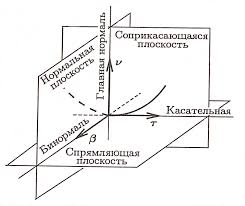
\includegraphics[]{img/images.jpeg}
                    \end{center}
                    \vspace{5px}

                    \define Предельное положение плоскости проходящее через точки $M_1,M_2$ некоторой траектории при стремлении $M_1,M_2 \to M$ называется \textbf{\textit{соприкасающейся плоскостью}}.

                    \vspace{5px}

                    \define Предельное положение прямой проходящей через точки $M,M_1$ при $M_1 \to M$ называется \textbf{\textit{касательной к траектории в точке M}}.Касательная лежит в соприкасающейся плоскости.

                    \vspace{5px}

                    \define Плоскость перпендикулярная касательной называется \textbf{\textit{нормальной}}.

                    \vspace{5px}

                    \define Прямая перпендикулярная касательной и лежащая в соприкасающейся плоскости называется \textbf{\textit{главной нормалью.}}

                    \vspace{5px}

                    \define Прямая перпендикулярная касательной и главной нормали называется \textbf{\textit{би-нормалью}}.

                    \vspace{5px}

                    \textit{$\tau$ выбирают в направлении движения точки, единичный вектор нормали $\vec n$ направлен в сторону вогнутости траектории, а единичный вектор $\vec b$ - би-нормаль направлен так, чтобы $\vec \tau, \vec n, \vec b$ образовывали правую тройку векторов.}

                    \vspace{5px}

                    \define Плоскость проходящая через касательную и би-нормаль называется \textbf{\textit{спрямляющей плоскостью}}.

                    \vspace{5px}

                    \define  Набор векторов $\vec \tau, \vec n, \vec b$ носит название \textbf{\textit{естественного трехгранника}}.


                    \begin{center}
                        \definecolor{qqwuqq}{rgb}{0,0.39,0}
                        \definecolor{xdxdff}{rgb}{0.49,0.49,1}
                        \begin{tikzpicture}[line cap=round,line join=round,>=triangle 45,x=1.0cm,y=0.8478959000681695cm]
                            \clip(39.05,145.94) rectangle (50.34,152.51);
                            \draw [shift={(47.32,151.4)},color=qqwuqq,fill=qqwuqq,fill opacity=0.1] (0,0) -- (-41.04:0.55) arc (-41.04:0.61:0.55) -- cycle;
                            \draw [->] (12,16) -- (12,30);
                            \draw [->] (12,16) -- (24,16);
                            \draw [->] (12,16) -- (6.1,10.4);
                            \draw [dash pattern=on 1pt off 1pt] (12,28)-- (18,24);
                            \draw [dash pattern=on 1pt off 1pt] (18,24)-- (18,12);
                            \draw [dash pattern=on 1pt off 1pt] (18,12)-- (7.8,12.01);
                            \draw [dash pattern=on 1pt off 1pt] (18,12)-- (22,16);
                            \draw [dash pattern=on 1pt off 1pt] (12,16)-- (18,24);
                            \draw (11.69,29.99) node[anchor=north west] {\textit{z}};
                            \draw (23.54,15.8) node[anchor=north west] {$y$};
                            \draw (6.51,10.99) node[anchor=north west] {$x$};
                            \draw (9.71,28.52) node[anchor=north west] {$z(t)$};
                            \draw (22.37,18.04) node[anchor=north west] {$x(t)$};
                            \draw (5.85,14.04) node[anchor=north west] {$y(t)$};
                            \draw [dash pattern=on 1pt off 1pt] (12,16)-- (18,12);
                            \draw (11.81,15.71) node[anchor=north west] {$O$};
                            \draw [shift={(37.64,72.37)}] plot[domain=0.31:2.77,variable=\t]({1*4.99*cos(\t r)+0*4.99*sin(\t r)},{0*4.99*cos(\t r)+1*4.99*sin(\t r)});
                            \draw (33.95,78.11) node[anchor=north west] {$M_0$};
                            \draw (40.77,77.73) node[anchor=north west] {$M$};
                            \draw (34.57,76.3)-- (40.92,76.13);
                            \draw (40.92,76.13)-- (37.52,69.39);
                            \draw (37.52,69.39)-- (34.57,76.3);
                            \draw (34.72,73.26) node[anchor=north west] {$\vec r_0$};
                            \draw (40.33,73.44) node[anchor=north west] {$\vec r$};
                            \draw (37.33,75.38) node[anchor=north west] {$\Delta \vec r$};
                            \draw [shift={(43.66,124.16)}] plot[domain=0.04:3.18,variable=\t]({1*3.67*cos(\t r)+0*3.67*sin(\t r)},{0*3.67*cos(\t r)+1*3.67*sin(\t r)});
                            \draw [dash pattern=on 1pt off 1pt] (40.01,122.87)-- (40,128);
                            \draw [->] (40,124) -- (43.61,127.82);
                            \draw [->] (40,124) -- (46.05,126.94);
                            \draw [->] (40,124) -- (41.53,127.14);
                            \draw [->] (40,124) -- (40,126.26);
                            \draw (43.08,129.35) node[anchor=north west] {$\Delta S$};
                            \draw (43.44,125.38) node[anchor=north west] {$\Delta \vec r$};
                            \draw (39.03,125.67) node[anchor=north west] {$\vec \tau$};
                            \draw(42.33,148.15) ellipse (1.89cm and 1.6cm);
                            \draw [shift={(42.13,147.3)}] plot[domain=0.32:3.37,variable=\t]({1*2.73*cos(\t r)+0*2.73*sin(\t r)},{0*2.73*cos(\t r)+1*2.73*sin(\t r)});
                            \draw [shift={(46.52,148.54)}] plot[domain=3.35:5.92,variable=\t]({1*1.84*cos(\t r)+0*1.84*sin(\t r)},{0*1.84*cos(\t r)+1*1.84*sin(\t r)});
                            \draw [->] (47.32,151.4) -- (49.44,151.43);
                            \draw [->] (47.32,151.4) -- (49.24,149.73);
                            \draw [->] (42.18,150.03) -- (44.27,150.16);
                            \draw [->] (42.33,148.15) -- (42.18,150.03);
                            \draw [->] (44.06,149.23) -- (45.55,147.95);
                            \draw (48.07,151.52) node[anchor=north west] {$\Delta \Theta$};
                            \draw (48.04,152.51) node[anchor=north west] {$\vec \tau_1$};
                            \draw (47.54,150.77) node[anchor=north west] {$\vec \tau_2$};
                            \draw (44.78,149.55) node[anchor=north west] {$\vec \tau_2$};
                            \draw (42.53,149.51) node[anchor=north west] {$\rho$};
                            \draw (42.97,151.22) node[anchor=north west] {$\vec \tau_1$};
                            \draw (41.91,151.54) node[anchor=north west] {$M$};
                            \draw (44.34,150.3) node[anchor=north west] {$M_1$};
                            \begin{scriptsize}
                                \fill [color=black] (12,16) circle (1.5pt);
                                \fill [color=black] (18,24) circle (1.5pt);
                                \draw[color=black] (38.8,156.71) node {$M$};
                                \fill [color=xdxdff] (34.57,76.3) circle (1.5pt);
                                \fill [color=xdxdff] (40.92,76.13) circle (1.5pt);
                                \fill [color=black] (42.18,150.03) circle (1.5pt);
                                \fill [color=black] (44.09,149.2) circle (1.5pt);
                            \end{scriptsize}
                        \end{tikzpicture}
                    \end{center}

                    \define  Угол $\Delta \Theta$ называют \textbf{\textit{углом дельта смежности}}.

                    \vspace{5px}

                    \define  Отношение $\frac{\Delta \Theta}{\Delta S}$ называют \textbf{\textit{средней кривизной траектории}}.Рассмотрим предел $\lim{\Delta s \to 0} \frac{\Delta \Theta}{\Delta s} = K$(параметр характеризующий траекторию) - \textbf{\textit{кривизна траектории}} в точке М($\frac{d \Theta}{ds} = K$)

                    \vspace{5px}

                    Выбираем три точки $M_1, M_2, M$ и проведем через них окружность (причем такая окружность единственна)

                    \vspace{5px}

                    \define  Предельное положение окружности при $M_1,M_2 \to M$ называют \textbf{\textit{кругом кривизны}}. Радиус такого круга называют \textbf{\textit{радиусом кривизны траектории}} в точке М и обозначается $\rho$. Причем имеет место соотношение
                    \begin{equation} \label{eq:kriv}
                        K = \frac{1}{\rho}
                    \end{equation}
              \item \underline{Естественный способ:}

                    \begin{center}
                        \definecolor{xdxdff}{rgb}{0.49,0.49,1}
                        \begin{tikzpicture}[line cap=round,line join=round,>=triangle 45,x=0.7956531517011031cm,y=0.6757341166288451cm]
                            \clip(40.74,146.55) rectangle (50.52,152.71);
                            \draw [->] (12,16) -- (12,30);
                            \draw [->] (12,16) -- (24,16);
                            \draw [->] (12,16) -- (6.1,10.4);
                            \draw [dash pattern=on 1pt off 1pt] (12,28)-- (18,24);
                            \draw [dash pattern=on 1pt off 1pt] (18,24)-- (18,12);
                            \draw [dash pattern=on 1pt off 1pt] (18,12)-- (7.8,12.01);
                            \draw [dash pattern=on 1pt off 1pt] (18,12)-- (22,16);
                            \draw [dash pattern=on 1pt off 1pt] (12,16)-- (18,24);
                            \draw (11.69,29.99) node[anchor=north west] {\textit{z}};
                            \draw (23.54,15.8) node[anchor=north west] {$y$};
                            \draw (6.51,10.99) node[anchor=north west] {$x$};
                            \draw (9.71,28.52) node[anchor=north west] {$z(t)$};
                            \draw (22.37,18.04) node[anchor=north west] {$x(t)$};
                            \draw (5.85,14.04) node[anchor=north west] {$y(t)$};
                            \draw [dash pattern=on 1pt off 1pt] (12,16)-- (18,12);
                            \draw (11.81,15.71) node[anchor=north west] {$O$};
                            \draw [shift={(37.64,72.37)}] plot[domain=0.31:2.77,variable=\t]({1*4.99*cos(\t r)+0*4.99*sin(\t r)},{0*4.99*cos(\t r)+1*4.99*sin(\t r)});
                            \draw (33.95,78.11) node[anchor=north west] {$M_0$};
                            \draw (40.77,77.73) node[anchor=north west] {$M$};
                            \draw (34.57,76.3)-- (40.92,76.13);
                            \draw (40.92,76.13)-- (37.52,69.39);
                            \draw (37.52,69.39)-- (34.57,76.3);
                            \draw (34.72,73.26) node[anchor=north west] {$\vec r_0$};
                            \draw (40.33,73.44) node[anchor=north west] {$\vec r$};
                            \draw (37.33,75.38) node[anchor=north west] {$\Delta \vec r$};
                            \draw [shift={(43.66,124.16)}] plot[domain=0.04:3.18,variable=\t]({1*3.67*cos(\t r)+0*3.67*sin(\t r)},{0*3.67*cos(\t r)+1*3.67*sin(\t r)});
                            \draw [dash pattern=on 1pt off 1pt] (40.01,122.87)-- (40,128);
                            \draw [->] (40,124) -- (43.61,127.82);
                            \draw [->] (40,124) -- (46.05,126.94);
                            \draw [->] (40,124) -- (41.53,127.14);
                            \draw [->] (40,124) -- (40,126.26);
                            \draw (43.08,129.35) node[anchor=north west] {$\Delta S$};
                            \draw (43.44,125.38) node[anchor=north west] {$\Delta \vec r$};
                            \draw (39.03,125.67) node[anchor=north west] {$\vec \tau$};
                            \draw [shift={(45.46,147.42)}] plot[domain=0.02:3.16,variable=\t]({1*4.58*cos(\t r)+0*4.58*sin(\t r)},{0*4.58*cos(\t r)+1*4.58*sin(\t r)});
                            \draw [->] (42.17,150.61) -- (43.61,152.51);
                            \draw [->] (42.17,150.61) -- (44.2,149.08);
                            \draw [->] (43.61,152.51) -- (44.2,149.08);
                            \draw (42.4,152.6) node[anchor=north west] {$\vec \tau_1$};
                            \draw (42.6,149.94) node[anchor=north west] {$\vec \tau_2$};
                            \draw (44.19,151.49) node[anchor=north west] {$\Delta \vec \tau$};
                            \draw (42.57,151.2) node[anchor=north west] {$\Delta \Theta$};
                            \draw [->] (48.43,150.91) -- (50.34,149.33);
                            \draw (49.21,151.22) node[anchor=north west] {$\vec \tau_2$};
                            \draw (42.62,151.74)-- (43,151.43);
                            \draw (43.28,150.07)-- (43.02,149.6);
                            \draw (41.74,151.7) node[anchor=north west] {$M$};
                            \draw (48.4,151.9) node[anchor=north west] {$M_1$};
                            \begin{scriptsize}
                                \fill [color=black] (12,16) circle (1.5pt);
                                \fill [color=black] (18,24) circle (1.5pt);
                                \draw[color=black] (40.57,157.19) node {$M$};
                                \fill [color=xdxdff] (34.57,76.3) circle (1.5pt);
                                \fill [color=xdxdff] (40.92,76.13) circle (1.5pt);
                                \fill [color=black] (48.43,150.91) circle (1.5pt);
                                \fill [color=black] (42.17,150.61) circle (1.5pt);
                            \end{scriptsize}
                        \end{tikzpicture}
                    \end{center}

                    \[\vec w = \frac{d(\vec \tau \cdot v)}{dt} = v\cdot \frac{d \vec \tau}{dt} + \vec \tau\cdot \frac{dv}{dt}\]

                    Рассмотрим, \[ \frac{d \vec \tau}{dt} = \lim_{\Delta t \to 0}  \frac{\Delta \vec \tau}{\Delta t}\]

                    При стремлении угла между $\tau_1$ и $\tau_2$ к нулю, угол между $\tau$ и $\Delta \vec \tau$ стремится к 90 градусам, то есть $\Delta \vec \tau$ сонаправлен с \textit{главной нормалью траектории движения}.

                    Из треугольника образованного векторами $\tau_1, \tau_2$ и $\Delta \vec \tau$ и того что:
                    \[|\Delta \tau| = 2 |\vec \tau| \cdot \sin{\frac{\Delta \Theta}{2}} = 2\sin{\frac{\Delta \Theta}{2}}\]
                    получаем что: \[ \lim_{\Delta t \to 0}  \frac{|\Delta \tau|}{\Delta t} = \lim_{\Delta t \to 0}  \frac{2sin(\frac{\Delta \Theta}{2})}{\Delta t} =
                        \lim_{\Delta t \to 0}  \frac{\Delta \Theta}{\frac{\Delta \Theta}{2}}\cdot\frac{\sin{\frac{\Delta \Theta}{2}}}{\Delta t}\cdot\frac{\Delta S}{\Delta S} \]
                    Устремим,
                    \[ \langle \Delta t \to 0 ;\Delta \Theta \to 0; \Delta S \to 0 \rangle = \]

                    \[ \lim_{\Delta \Theta \to 0}  \frac{\sin{\frac{\Delta \Theta}{2}}}{\frac{\Delta \Theta}{2}} \cdot \lim_{\Delta S \to 0} \frac{\Delta \Theta}{\Delta S} \cdot \lim_{\Delta t \to 0} \frac{\Delta S}{\Delta t} \]
                    Так как,
                    \[ \langle \lim_{\Delta \Theta \to 0}  \frac{\sin{\frac{\Delta \Theta}{2}}}{\frac{\Delta \Theta}{2}} \to 1 ; \lim_{\Delta S \to 0} \frac{\Delta \Theta}{\Delta S} \to k; \lim_{\Delta t \to 0} \frac{\Delta S}{\Delta t} \to v \rangle \]
                    % \[ k \cdot v = \frac{v}{\rho} \text{\begin{flushright}(следует из \hyperref[eq:kriv]{(\ref{eq:kriv})} )\end{flushright}}\] %TODO!: Чёт не работает, фиксануть

                    \vspace{5px}

                    То есть \[\frac{d \tau}{dt} = \vec n \cdot \frac{v}{\rho}. \]
                    Таким образом,\[ \vec w = \frac{v^2}{\rho} \cdot \vec n + \vec \tau \cdot \frac{dv}{dt} = \vec w_n + \vec w_\tau \]где $\frac{v^2}{p} \cdot \vec n$  - нормальная составляющая ускорения и $\vec \tau \cdot \frac{dv}{dt}$ - тангенциальное ускорение.

                    \vspace{5px}

                    Вывод:

                    \[ w = \sqrt{w_n^2 +w_\tau^2}\] где $ \tan{\phi} = \frac{w_\tau}{w_n}$ , следовательно, тангенциальное ускорение:  \[ w_\tau = \tan{\phi} \cdot w_n\]

                    \begin{center}
                        \definecolor{xdxdff}{rgb}{0.49,0.49,1}
                        \begin{tikzpicture}[line cap=round,line join=round,>=triangle 45,x=0.7295609638745411cm,y=0.5944748450860953cm]
                            \clip(42.02,150.24) rectangle (49.41,155.17);
                            \draw[fill=black,fill opacity=0.05] (45.52,153.53) -- (46.04,153.57) -- (46,154.09) -- (45.48,154.05) -- cycle;
                            \draw [shift={(45.48,154.05)}] (0,0) -- (-85.73:0.99) arc (-85.73:-44.47:0.99) -- cycle;
                            \draw [->] (12,16) -- (12,30);
                            \draw [->] (12,16) -- (24,16);
                            \draw [->] (12,16) -- (6.1,10.4);
                            \draw [dash pattern=on 1pt off 1pt] (12,28)-- (18,24);
                            \draw [dash pattern=on 1pt off 1pt] (18,24)-- (18,12);
                            \draw [dash pattern=on 1pt off 1pt] (18,12)-- (7.8,12.01);
                            \draw [dash pattern=on 1pt off 1pt] (18,12)-- (22,16);
                            \draw [dash pattern=on 1pt off 1pt] (12,16)-- (18,24);
                            \draw (11.67,30.11) node[anchor=north west] {\textit{z}};
                            \draw (23.55,15.89) node[anchor=north west] {$y$};
                            \draw (6.5,11.08) node[anchor=north west] {$x$};
                            \draw (9.7,28.62) node[anchor=north west] {$z(t)$};
                            \draw (22.37,18.14) node[anchor=north west] {$x(t)$};
                            \draw (5.83,14.13) node[anchor=north west] {$y(t)$};
                            \draw [dash pattern=on 1pt off 1pt] (12,16)-- (18,12);
                            \draw (11.75,15.62) node[anchor=north west] {$O$};
                            \draw [shift={(37.64,72.37)}] plot[domain=0.31:2.77,variable=\t]({1*4.99*cos(\t r)+0*4.99*sin(\t r)},{0*4.99*cos(\t r)+1*4.99*sin(\t r)});
                            \draw (33.93,78.21) node[anchor=north west] {$M_0$};
                            \draw (40.79,77.81) node[anchor=north west] {$M$};
                            \draw (34.57,76.3)-- (40.92,76.13);
                            \draw (40.92,76.13)-- (37.52,69.39);
                            \draw (37.52,69.39)-- (34.57,76.3);
                            \draw (34.72,73.37) node[anchor=north west] {$\vec r_0$};
                            \draw (40.34,73.52) node[anchor=north west] {$\vec r$};
                            \draw (37.33,75.47) node[anchor=north west] {$\Delta \vec r$};
                            \draw [shift={(43.66,124.16)}] plot[domain=0.04:3.18,variable=\t]({1*3.67*cos(\t r)+0*3.67*sin(\t r)},{0*3.67*cos(\t r)+1*3.67*sin(\t r)});
                            \draw [dash pattern=on 1pt off 1pt] (40.01,122.87)-- (40,128);
                            \draw [->] (40,124) -- (43.61,127.82);
                            \draw [->] (40,124) -- (46.05,126.94);
                            \draw [->] (40,124) -- (41.53,127.14);
                            \draw [->] (40,124) -- (40,126.26);
                            \draw (43.08,129.45) node[anchor=north west] {$\Delta S$};
                            \draw (43.45,125.49) node[anchor=north west] {$\Delta \vec r$};
                            \draw (39.04,125.76) node[anchor=north west] {$\vec \tau$};
                            \draw [shift={(45.74,150.84)}] plot[domain=0.08:3.22,variable=\t]({1*3.22*cos(\t r)+0*3.22*sin(\t r)},{0*3.22*cos(\t r)+1*3.22*sin(\t r)});
                            \draw [->] (45.48,154.05) -- (45.68,151.43);
                            \draw [->] (45.48,154.05) -- (47.7,154.21);
                            \draw [dash pattern=on 1pt off 1pt] (45.68,151.43)-- (47.94,151.63);
                            \draw [dash pattern=on 1pt off 1pt] (47.7,154.21)-- (47.94,151.63);
                            \draw [->] (45.48,154.05) -- (47.94,151.63);
                            \draw (46.01,153.04) node[anchor=north west] {$\phi$};
                            \draw (46.26,155.29) node[anchor=north west] {$\vec w_\tau$};
                            \draw (44.8,153.19) node[anchor=north west] {$\vec w_n$};
                            \draw (48.06,151.79) node[anchor=north west] {$\vec w$};
                            \begin{scriptsize}
                                \fill [color=black] (12,16) circle (1.5pt);
                                \fill [color=black] (18,24) circle (1.5pt);
                                \draw[color=black] (39.38,158.7) node {$M$};
                                \fill [color=xdxdff] (34.57,76.3) circle (1.5pt);
                                \fill [color=xdxdff] (40.92,76.13) circle (1.5pt);
                            \end{scriptsize}
                        \end{tikzpicture}
                    \end{center}

          \end{enumerate}
\end{enumerate}
\textbf{\textit{!!!Важно : При движении по кривой из v = const не следует, что w=0(например, движение по окружности)}} %TODO: Фиксануть переполнение

\section{Частные случаи движения точек}
\subsection{Прямолинейное движение точки}
\define  Если траектория движения точки является частью прямой линии, такое движение называется \textbf{\textit{прямолинейным}}. В этом движении систему координат выбирают так, чтобы траектория движения лежала на одной из осей декартовой системы координат.

\vspace{5px}

Координаты на одной из осей всегда будут нулевыми, так движение точки будет описываться с помощью одной координаты. Тогда $ v(t) = \frac{df}{dt}, w =\frac{dv}{dt}$,  а направление вектора скорости соответственно будет определяться по знаку: ( + ) --- в направлении оси,( - ) --- в противоположном направлении.
\begin{enumerate}
    \item \textit{равномерное движение} $v - const; x = v \cdot t + x_0 $
    \item \textit{равнопеременное движение} $w - const; w = a$
          $\frac{dv}{dt} = a => v = a \cdot t + C $ где С находится из начального условия $v(0) = v_0$, то есть:
          \[ v = at+v_0\]
          %   \[ x = \frac{at^2}{2} + v_0t+ C \text{\begin{flushright} , где С = $x_0 (x(0) = x_0)$ \end{flushright}}\] %TODO!: Фиксануть формул.
\end{enumerate}

\vspace{10px}

\textbf{Колебательное движение}

% \[ x = A \cdot \sin{(\omega t+ \phi_0)} \text{,где \begin{flushright} $\phi_0$ - начальная фаза\end{flushright}}\] %TODO!: Фикс фикса
\[ v = A \cdot \cos{(\omega t+ \phi_0)}\]
\[ W = -A\omega ^2 \cdot \sin{(\omega t+\phi_0)} = -\omega^2x \]
\textit{Если знаки $v(t) , W(t)$ совпадают, то движение ускоренное, если нет - замедленное.}
\subsection{Круговое движение}


\begin{center}
    \definecolor{xdxdff}{rgb}{0.49,0.49,1}
    \begin{tikzpicture}[line cap=round,line join=round,>=triangle 45,x=0.6693000916944117cm,y=0.6542364468628811cm]
        \clip(41.72,143.75) rectangle (50.79,152.43);
        \draw [shift={(46.04,147.65)}] (0,0) -- (11.38:0.74) arc (11.38:90.81:0.74) -- cycle;
        \draw [->] (12,16) -- (12,30);
        \draw [->] (12,16) -- (24,16);
        \draw [->] (12,16) -- (6.1,10.4);
        \draw [dash pattern=on 2pt off 2pt] (12,28)-- (18,24);
        \draw [dash pattern=on 2pt off 2pt] (18,24)-- (18,12);
        \draw [dash pattern=on 2pt off 2pt] (18,12)-- (7.8,12.01);
        \draw [dash pattern=on 2pt off 2pt] (18,12)-- (22,16);
        \draw [dash pattern=on 2pt off 2pt] (12,16)-- (18,24);
        \draw (11.67,30.11) node[anchor=north west] {\textit{z}};
        \draw (23.55,15.89) node[anchor=north west] {$y$};
        \draw (6.5,11.08) node[anchor=north west] {$x$};
        \draw (9.7,28.62) node[anchor=north west] {$z(t)$};
        \draw (22.37,18.14) node[anchor=north west] {$x(t)$};
        \draw (5.83,14.13) node[anchor=north west] {$y(t)$};
        \draw [dash pattern=on 2pt off 2pt] (12,16)-- (18,12);
        \draw (11.75,15.62) node[anchor=north west] {$O$};
        \draw [shift={(37.64,72.37)}] plot[domain=0.31:2.77,variable=\t]({1*4.99*cos(\t r)+0*4.99*sin(\t r)},{0*4.99*cos(\t r)+1*4.99*sin(\t r)});
        \draw (33.93,78.21) node[anchor=north west] {$M_0$};
        \draw (40.79,77.81) node[anchor=north west] {$M$};
        \draw (34.57,76.3)-- (40.92,76.13);
        \draw (40.92,76.13)-- (37.52,69.39);
        \draw (37.52,69.39)-- (34.57,76.3);
        \draw (34.72,73.37) node[anchor=north west] {$\bar r_0$};
        \draw (40.34,73.52) node[anchor=north west] {$\vec r$};
        \draw (37.33,75.47) node[anchor=north west] {$\Delta \vec r$};
        \draw [shift={(43.66,124.16)}] plot[domain=0.04:3.18,variable=\t]({1*3.67*cos(\t r)+0*3.67*sin(\t r)},{0*3.67*cos(\t r)+1*3.67*sin(\t r)});
        \draw [dash pattern=on 2pt off 2pt] (40.01,122.87)-- (40,128);
        \draw [->] (40,124) -- (43.61,127.82);
        \draw [->] (40,124) -- (46.05,126.94);
        \draw [->] (40,124) -- (41.53,127.14);
        \draw [->] (40,124) -- (40,126.26);
        \draw (43.08,129.45) node[anchor=north west] {$\Delta S$};
        \draw (43.45,125.49) node[anchor=north west] {$\Delta \vec r$};
        \draw (39.04,125.76) node[anchor=north west] {$\vec \tau$};
        \draw(46.04,147.65) ellipse (2.34cm and 2.29cm);
        \draw (48.45,151.55) node[anchor=north west] {$S$};
        \draw (50.03,149.23) node[anchor=north west] {$M$};
        \draw (45.77,152.49) node[anchor=north west] {$M_0$};
        \draw [->] (46.04,147.65) -- (45.99,151.15);
        \draw [->] (46.04,147.65) -- (49.47,148.34);
        \draw (45.2,150.12) node[anchor=north west] {$\vec r_0$};
        \draw (47.44,148.08) node[anchor=north west] {$\vec r$};
        \draw (45.2,146.59) node[anchor=north west] {$| \Delta r | \neq \Delta | r |$};
        \draw (46.63,149.54) node[anchor=north west] {$\phi$};
        \begin{scriptsize}
            \fill [color=black] (12,16) circle (1.5pt);
            \fill [color=black] (18,24) circle (1.5pt);
            \draw[color=black] (39.38,158.7) node {$M$};
            \fill [color=xdxdff] (34.57,76.3) circle (1.5pt);
            \fill [color=xdxdff] (40.92,76.13) circle (1.5pt);
            \fill [color=black] (45.99,151.15) circle (1.5pt);
            \fill [color=black] (49.47,148.34) circle (1.5pt);
        \end{scriptsize}
    \end{tikzpicture}
\end{center}


\define \textit{Если траектория движения точки является частью некоторой окружности, то движение называется \textbf{круговым}.}

\vspace{5px}

\define  Путь $s(t) = \phi(t) \cdot R $
\[ v(t) = \frac{ds}{dt} = R \cdot \frac{d\phi}{dt}\]
где $\frac{d\phi}{dt}$ называется \textbf{\textit{угловой скоростью}} и обозначается $\omega (v = R\omega)$
\[ w_\tau = \frac{dv}{dt} = R \cdot \frac{d^2 \phi}{dt} = R \cdot \frac{dw}{dt} \]
где  $\frac{dw}{dt}$ называется угловым ускорением и обозначается $\epsilon$
\[ w_\tau = R \cdot \epsilon \text{ --- \textbf{\textit{касательное ускорение}}} \]
\[w_n = \frac{v^2}{R} = \omega^2 \cdot R \text{ --- \textbf{\textit{нормальное ускорение}}} \]
\[ \vec w = \vec w_\tau + \vec w_n\]
\[ w = R \sqrt{w_n^4 + \epsilon^2} \]
\section{Кинематика системы материальных точек и твердого тела}
\define  На систему материальных точек могут быть наложены ограничения, называемые связями. Для однозначного задания системы из n точек необходимо задать 3n координат.

\vspace{5px}

---Если связи наложены только на координаты материальных точек, то они называются \textbf{\textit{геометрическими}}.

\vspace{5px}

---Если связи наложены на координаты и скорости точек,то такие связи называются \textbf{\textit{кинематическими}}. Связи могут быть выражены уравнениями.
\begin{itemize}
    \item Для геометрической связи: $f_0 = f(x_1,y_1,z_1, \dots , x_n, y_n, z_n)$
    \item Для кинематической связи: $g_0 = g(x_1,y_1,z_1, \dots , x_n, y_n, z_n, \dot x_1,\dot y_1,\dot z_1, \dots , \dot x_n, \dot y_n,\dot z_n)$ %TODO: Переполнение hbox
\end{itemize}
Это уравнения для системы из n материальных точек.

\vspace{5px}

\define \textit{Если на систему наложено \texttt{К} связей, определенные уравнениями, то независимыми координатами будут только \texttt{3n - K} координат. Они называются координатами системы.}

\vspace{5px}

\define Если на систему наложены только геометрические связи, то количество координат системы называется \textbf{\textit{числом степеней свободы системы}}.

\vspace{5px}

В абсолютно твердом теле расстояние между любыми двумя точками неизменно. Абсолютно твердое тело имеет 6 степеней свободы.

\vspace{6px}

\textbf{Докажем данное утверждение:} возьмем в твердом теле точку $ A(x_A,y_A,z_A)$. Затем точку $ B(x_{B},y_{B},z_{B})$ и добавим связь \[ r_{AB} = \sqrt{(x_A-x_B)^2 + (y_A-y_B)^2 + (z_A-z_B)^2} = const \]
Это уравнение накладывает одну связь между координатами $x_B, y_B,z_B$, то есть уменьшает количество независимых координат с 3 до 2.

Итого для описания положения точек A и B нужно 3+2 = 5 независимых координат

Возьмем аналогично точку $ С(x_{С},y_{С},z_{С})$ и добавим две связи : \[ r_{AC} = const, r_{BC} = const \] %TODO: Инвалид что-го то там

Получим 9 координат и уже 3 связи:
\[r_{AB} = const\]
\[r_{AC} = const\]
\[r_{BC} = const\]

Эти связи уменьшают число независимых координат точки С с 3 до 1.Итого для описания положения точек A, B, C теперь нужно 3+2+1 = 6 независимых координат.

Возьмем точку $D(x_0,y_0,z_0)$ , вместе с ней добавятся и 3 связи
\[ r_{AD} = const\]
\[ r_{CD} = const\]
\[ r_{BD} = const\]

Эти связи полностью фиксируют положение точки D и они больше не добавляют степеней свободы(независимых координат для описания)

Для любой другой точки число степеней свободы останется прежним, они также жоско привязаны к первой точке А и поэтому не увеличивают общее число степеней свободы.

\section{Координаты свободного твердого тела, углы Эйлера}


\begin{center}
    \definecolor{ffqqqq}{rgb}{1,0,0}
    \definecolor{qqqqff}{rgb}{0,0,1}
    \begin{tikzpicture}[line cap=round,line join=round,>=triangle 45,x=0.28919850580791134cm,y=0.28489474787983016cm]
        \clip(4.64,7.06) rectangle (54.06,31.63);
        \draw [shift={(35,15)}] (0,0) -- (90:2.41) arc (90:116.57:2.41) -- cycle;
        \draw [shift={(35,15)},color=ffqqqq] (0,0) -- (-18.43:3.21) arc (-18.43:63.43:3.21) -- cycle;
        \draw [shift={(35,15)},color=qqqqff] (0,0) -- (-135:3.21) arc (-135:-18.43:3.21) -- cycle;
        \draw [->] (11.86,15.08) -- (12,30);
        \draw [->] (11.86,15.08) -- (23.79,15.13);
        \draw [->] (11.86,15.08) -- (6.33,10.57);
        \draw (11.7,30.93) node[anchor=north west] {\textit{z}};
        \draw (23.57,16.77) node[anchor=north west] {$y$};
        \draw (6.48,11.91) node[anchor=north west] {$x$};
        \draw (10.17,29.84) node[anchor=north west] {$Z$};
        \draw (5.76,13.89) node[anchor=north west] {$X$};
        \draw (21.89,19.04) node[anchor=north west] {$Y$};
        \draw (11.06,13.79) node[anchor=north west] {$O$};
        \draw [shift={(17.32,24.36)}] plot[domain=0.49:3.05,variable=\t]({1*2.86*cos(\t r)+0*2.86*sin(\t r)},{0*2.86*cos(\t r)+1*2.86*sin(\t r)});
        \draw [shift={(17.66,25.72)}] plot[domain=4.07:6.28,variable=\t]({1*2.19*cos(\t r)+0*2.19*sin(\t r)},{0*2.19*cos(\t r)+1*2.19*sin(\t r)});
        \draw [shift={(15.49,24.52)}] plot[domain=3.02:5.71,variable=\t]({1*1.02*cos(\t r)+0*1.02*sin(\t r)},{0*1.02*cos(\t r)+1*1.02*sin(\t r)});
        \draw [->] (16.18,25.66) -- (16.12,30.93);
        \draw [->] (16.18,25.66) -- (23.45,25.65);
        \draw [->] (16.18,25.66) -- (11.49,21.74);
        \draw (16.11,26.57) node[anchor=north west] {$A$};
        \draw (21.57,29.15) node[anchor=north west] {$x_A$};
        \draw (13.14,26.38) node[anchor=north west] {$y_A$};
        \draw (16.83,32.22) node[anchor=north west] {$z_A$};
        \draw [->] (35,15) -- (35,30);
        \draw [->] (35,15) -- (30,10);
        \draw [->] (35,15) -- (50,15);
        \draw [->] (35,15) -- (40,10);
        \draw [->] (35,15) -- (50,10);
        \draw [->] (35,15) -- (40,25);
        \draw [->] (35,15) -- (30,25);
        \draw [shift={(35,15)}] (90:2.41) arc (90:116.57:2.41);
        \draw [shift={(35,15)}] (90:2.01) arc (90:116.57:2.01);
        \draw [shift={(35,15)},color=qqqqff] (-135:3.21) arc (-135:-18.43:3.21);
        \draw [shift={(35,15)},color=qqqqff] (-135:2.81) arc (-135:-18.43:2.81);
        \draw [shift={(35,15)},color=qqqqff] (-135:2.41) arc (-135:-18.43:2.41);
        \draw (33.6,20.33) node[anchor=north west] {$\Theta$};
        \draw (37.93,20.13) node[anchor=north west] {$\psi$};
        \draw (33.84,12.6) node[anchor=north west] {$\phi$};
        \draw (29.83,12.9) node[anchor=north west] {$X$};
        \draw (35.36,30.93) node[anchor=north west] {$Z$};
        \draw (48.92,17.95) node[anchor=north west] {$Y$};
        \draw [dash pattern=on 1pt off 1pt on 2pt off 4pt] (40,25)-- (40,10);
        \draw (30.79,26.28) node[anchor=north west] {$\bar z$};
        \draw (38.73,26.57) node[anchor=north west] {$\bar y$};
        \draw (38.49,12.01) node[anchor=north west] {$\bar x$};
        \begin{scriptsize}
            \fill [color=black] (11.86,15.08) circle (1.5pt);
            \fill [color=qqqqff] (16.18,25.66) circle (1.5pt);
            \fill [color=black] (35,15) circle (1.5pt);
            \draw[color=black] (35.61,16.27) node {$O$};
        \end{scriptsize}
    \end{tikzpicture}
\end{center}
Берем точку твердого тела A. Затем к ней привязываем систему координат внутри тела, задающих ориентацию тела в пространстве. Используя параллельный перенос переместим точку А в точку О.
\begin{enumerate}
    \item при повороте измеряем углы поворота в $x_AOy_Az_A$.Совместим O и А образуется угол $\angle ZOz = \Theta$ - \textit{угол нутации.}
    \item Рассмотрим плоскость $xAy$ в пересечении с $XOY = ol$.

          $xAy \bigcap XOY = ol$ - \textit{линия узлов}

          $\angle XOl = \phi$ - \textit{угол прецессии}

          $\angle lAy = \psi$ - \textit{угол собственного вращения}
\end{enumerate}
Причем \[ 0 < \Theta \leq 180 , 0 < \phi \leq 360, 0 < \psi \leq 360 \]

\vspace{5px}

\textbf{Таким образом, эти углы однозначно определяют положение твердого тела в пространстве с помощью координат ($x_A, y_A, z_A, \Theta, \phi, \psi$), где $A(x_A, y_A,z_A)$ - полюс.} %TODO: Переполнение


\section{Простейшие формы движения твердого тела}
\subsection{Поступательное движение}
\begin{center}
    \definecolor{qqqqff}{rgb}{0,0,1}
    \begin{tikzpicture}[line cap=round,line join=round,>=triangle 45,x=0.3737271459851131cm,y=0.3189582101091683cm]
        \clip(5.52,9.54) rectangle (24.68,31.57);
        \draw [->] (11.86,15.08) -- (12,30);
        \draw [->] (11.86,15.08) -- (23.79,15.13);
        \draw [->] (11.86,15.08) -- (6.33,10.57);
        \draw (11.66,30.48) node[anchor=north west] {\textit{z}};
        \draw (23.55,16.28) node[anchor=north west] {$y$};
        \draw (6.5,11.43) node[anchor=north west] {$x$};
        \draw (10.14,29.39) node[anchor=north west] {$Z$};
        \draw (5.81,13.43) node[anchor=north west] {$X$};
        \draw (21.93,18.65) node[anchor=north west] {$Y$};
        \draw (11.37,14.28) node[anchor=north west] {$O$};
        \draw [shift={(17.32,24.36)}] plot[domain=0.49:3.05,variable=\t]({1*2.86*cos(\t r)+0*2.86*sin(\t r)},{0*2.86*cos(\t r)+1*2.86*sin(\t r)});
        \draw [shift={(17.66,25.72)}] plot[domain=4.07:6.28,variable=\t]({1*2.19*cos(\t r)+0*2.19*sin(\t r)},{0*2.19*cos(\t r)+1*2.19*sin(\t r)});
        \draw [shift={(15.49,24.52)}] plot[domain=3.02:5.71,variable=\t]({1*1.02*cos(\t r)+0*1.02*sin(\t r)},{0*1.02*cos(\t r)+1*1.02*sin(\t r)});
        \draw [->] (16.18,25.66) -- (16.12,30.93);
        \draw [->] (16.18,25.66) -- (23.45,25.65);
        \draw [->] (16.18,25.66) -- (11.49,21.74);
        \draw (16.08,26.17) node[anchor=north west] {$A$};
        \draw (21.54,28.66) node[anchor=north west] {$x_A$};
        \draw (13.13,25.93) node[anchor=north west] {$y_A$};
        \draw (16.87,31.75) node[anchor=north west] {$z_A$};
        \draw [->] (11.86,15.08) -- (16.18,25.66);
        \draw [->] (11.86,15.08) -- (23.11,25.65);
        \draw (13.18,22.47) node[anchor=north west] {$\vec r_0$};
        \draw (19.96,28.11) node[anchor=north west] {$\vec r^\prime$};
        \draw (17.7,23.08) node[anchor=north west] {$\vec r$};
        \begin{scriptsize}
            \fill [color=black] (11.86,15.08) circle (1.5pt);
            \fill [color=qqqqff] (16.18,25.66) circle (1.5pt);
            \fill [color=black] (23.11,25.65) circle (1.5pt);
            \draw[color=black] (23.55,26.41) node {$M$};
        \end{scriptsize}
    \end{tikzpicture}
\end{center}
При поступательном движении любой вектор проведенный в твердом теле остается параллелен самому себе. Очевидно: $\vec r = \vec r_0 + \vec r^\prime, r^\prime$ - проведенный вектор из т.А в конец вектора $r$ и за счет этого $| \vec r^\prime | - const$, причем направление этого вектора также не меняется , поскольку движение поступательное.

\vspace{5px}

Пример поступательного движения:
\begin{center}
    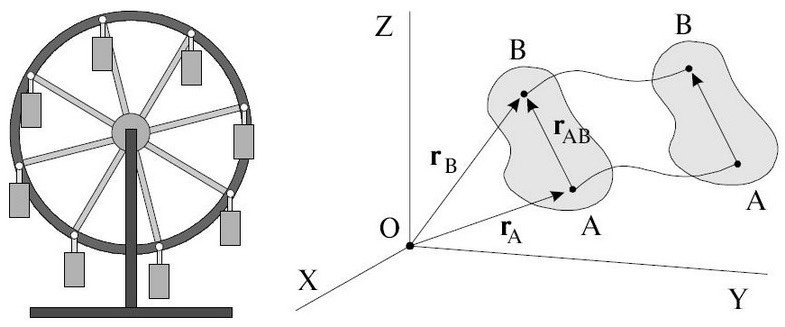
\includegraphics[width=8cm, height=3cm]{img/postup.jpg}
\end{center}
Траектории точек одинаковы, просто сдвиг на $r^\prime $, применим операцию дифференцирования к $r(t)$:
\[ \frac{dr}{dt} = \frac{dr_0}{dt} + \frac{dr^\prime}{dt} = 0 \Rightarrow v_M = v_A\]
Получаем что скорости точек А и М одинаковы, причем если мы еще раз продифференцируем это равенство получим что ускорения этих точек также равны.

\vspace{5px}

\textit{Для описания поступательного движения твердого тела достаточно описания движения лишь одной его точки.}


\subsection{Вращение твердого тела вокруг неподвижной оси}
Если при своем движении твердого тела 2 точки A и B не меняют своего положения, то говорят, что \textit{твердое тело вращается вокруг неподвижной оси}, проходящей через А и В, соответственно АВ - прямая являющаяся осью вращения.
\begin{center}
    \definecolor{fftttt}{rgb}{1,0.2,0.2}
    \definecolor{qqqqff}{rgb}{0,0,1}
    \definecolor{qqwuqq}{rgb}{0,0.39,0}
    \definecolor{qqqqcc}{rgb}{0,0,0.8}
    \begin{tikzpicture}[line cap=round,line join=round,>=triangle 45,x=1.0cm,y=1.0cm]
        \clip(7.98,22.58) rectangle (20.34,36.2);
        \draw [shift={(13,27)},color=qqwuqq,fill=qqwuqq,fill opacity=0.1] (0,0) -- (-143.13:0.6) arc (-143.13:-63.43:0.6) -- cycle;
        \draw [shift={(13,27)},line width=1.2pt,color=fftttt,fill=fftttt,fill opacity=0.1] (0,0) -- (71.57:1.2) arc (71.57:90:1.2) -- cycle;
        \draw [->] (13,27) -- (13,35);
        \draw [->] (13,27) -- (18,27);
        \draw [->] (13,27) -- (9,24);
        \draw [rotate around={100.82:(13.47,28.63)}] (13.47,28.63) ellipse (4.43cm and 1.96cm);
        \draw [->,color=qqqqcc] (13,27) -- (15,23);
        \draw [->,color=qqqqcc] (13,27) -- (17,32);
        \draw (15,23)-- (15,33);
        \draw (15,33)-- (13,34.11);
        \draw (13,34.11)-- (10,32.58);
        \draw (10,32.58)-- (10.03,24.77);
        \draw [rotate around={-0.63:(12.91,29.99)},dash pattern=on 3pt off 3pt] (12.91,29.99) ellipse (1.09cm and 0.6cm);
        \draw [->] (13,27) -- (14,30);
        \draw [->] (13.56,29.26) -- (14.4,30.6);
        \draw [dash pattern=on 3pt off 3pt] (14,30)-- (14,25);
        \draw (13.34,35.12) node[anchor=north west] {$z = z^\prime$};
        \draw (14,23.96) node[anchor=north west] {$x^\prime$};
        \draw (16.52,31.86) node[anchor=north west] {$y^\prime$};
        \draw (9.64,24.42) node[anchor=north west] {$x$};
        \draw (17.26,27.06) node[anchor=north west] {$y$};
        \draw (14,30)-- (13,30);
        \draw (13.36,30.62) node[anchor=north west] {$a$};
        \draw [shift={(13,27)},line width=1.2pt,color=fftttt] (71.57:1.2) arc (71.57:90:1.2);
        \draw [shift={(13,27)},line width=1.2pt,color=fftttt] (71.57:1.09) arc (71.57:90:1.09);
        \draw (14.28,30) node[anchor=north west] {$\vec w$};
        \draw (12.46,27.6) node[anchor=north west] {$O$};
        \begin{scriptsize}
            \fill [color=qqqqff] (14,30) circle (1.5pt);
            \fill [color=black] (13,30) circle (1.5pt);
            \draw[color=fftttt] (13.48,28.54) node {$\alpha$};
        \end{scriptsize}
    \end{tikzpicture}
\end{center}
Неподвижными точками будут и все точки на прямой АВ, то есть тело вращения имеет только одну степень свободы - достаточно лишь задать одну координату, чтобы определить положение тела в пространстве.

\vspace{5px}

$\phi(t) $ - функция определяющая положение тела в пространстве с помощью значения двухгранного угла, включающие отслеживаемую точку в разные моменты времени(причем траектория движения очевидно повторяет окружность)

\[ \alpha - const , a - const : a = r_M \cdot \sin{\alpha} \]
\[ \omega = \frac{d\phi}{dt} \]
\[ v = a \cdot \omega = r_M \cdot \sin{\alpha} \cdot \omega \] - причем вектор скорости будет направлен по оси вращения, формулы можем записать вектор скорости как $\vec v = [\omega, r] => \frac{dr}{dt} = [\omega,r]$. Так как $r - const$ такое равенство будет верно. Из этого выведем вектор ускорения:

\[ \vec w = \frac{dv}{dt} = \frac{d}{dt} [\vec \omega, \vec r] = [\frac{d\omega}{dt}, \vec r] + [\vec \omega, \frac{dr}{dt}] \] так как $\vec \omega$ - вектор, то и угловое ускорение $\vec \epsilon = \frac{d\omega}{dt}$ - вектор.

\vspace{5px}

Получаем :
\[ \vec w = \frac{d}{dt} [\vec \omega, \vec r] = [\frac{d\omega}{dt}, \vec r] + [\vec \omega, \frac{dr}{dt}] = [\vec \epsilon, \vec r] + [\vec \omega, \vec v]  = [\vec \epsilon, \vec r] + [\omega, [\omega,r]] \text{ ,где $ [\vec \epsilon, \vec r] = w_\tau $ , а  $[\omega, [\omega,r]] = w_n$}\] %TODO: Переполнение фиксануть

\subsection{Скорость и ускорение точек абсолютно твердого тела при сложном движении}
\begin{center}
    \definecolor{fftttt}{rgb}{1,0.2,0.2}
    \definecolor{qqqqff}{rgb}{0,0,1}
    \definecolor{qqwuqq}{rgb}{0,0.39,0}
    \definecolor{qqqqcc}{rgb}{0,0,0.8}
    \begin{tikzpicture}[line cap=round,line join=round,>=triangle 45,x=1.4791176048705874cm,y=1.8441311417483108cm]
        \clip(44.96,95.72) rectangle (49.13,99.28);
        \draw [shift={(13,27)},color=qqwuqq,fill=qqwuqq,fill opacity=0.1] (0,0) -- (-143.13:0.27) arc (-143.13:-63.43:0.27) -- cycle;
        \draw [shift={(13,27)},line width=1.2pt,color=fftttt,fill=fftttt,fill opacity=0.1] (0,0) -- (71.57:0.53) arc (71.57:90:0.53) -- cycle;
        \draw [->] (13,27) -- (13,35);
        \draw [->] (13,27) -- (18,27);
        \draw [->] (13,27) -- (9,24);
        \draw [rotate around={100.82:(13.47,28.63)}] (13.47,28.63) ellipse (6.55cm and 3.61cm);
        \draw [->,color=qqqqcc] (13,27) -- (15,23);
        \draw [->,color=qqqqcc] (13,27) -- (17,32);
        \draw (15,23)-- (15,33);
        \draw (15,33)-- (13,34.11);
        \draw (13,34.11)-- (10,32.58);
        \draw (10,32.58)-- (10.03,24.77);
        \draw [rotate around={-0.63:(12.91,29.99)},dash pattern=on 1pt off 1pt] (12.91,29.99) ellipse (1.61cm and 1.11cm);
        \draw [->] (13,27) -- (14,30);
        \draw [->] (13.56,29.26) -- (14.4,30.6);
        \draw [dash pattern=on 1pt off 1pt] (14,30)-- (14,25);
        \draw (13.34,34.99) node[anchor=north west] {$z = z^\prime$};
        \draw (14,23.83) node[anchor=north west] {$x^\prime$};
        \draw (16.52,31.73) node[anchor=north west] {$y^\prime$};
        \draw (9.64,24.29) node[anchor=north west] {$x$};
        \draw (17.26,26.92) node[anchor=north west] {$y$};
        \draw (14,30)-- (13,30);
        \draw (13.36,30.49) node[anchor=north west] {$a$};
        \draw [shift={(13,27)},line width=1.2pt,color=fftttt] (71.57:0.53) arc (71.57:90:0.53);
        \draw [shift={(13,27)},line width=1.2pt,color=fftttt] (71.57:0.48) arc (71.57:90:0.48);
        \draw (14.28,29.87) node[anchor=north west] {$\vec w$};
        \draw (12.46,27.46) node[anchor=north west] {$O$};
        \draw [->] (46,96.5) -- (46,99);
        \draw [->] (46,96.5) -- (45.5,96);
        \draw [->] (46,96.5) -- (48.5,96.5);
        \draw [rotate around={-8.45:(47.48,97.43)},fill=black,fill opacity=0.1] (47.48,97.43) ellipse (1.79cm and 0.96cm);
        \draw [->] (46,96.5) -- (47,97.5);
        \draw [->] (47,97.5) -- (47.01,98.59);
        \draw [->] (47,97.5) -- (48,97.5);
        \draw [->] (46,96.5) -- (48,97.5);
        \draw (46.65,98.29) node[anchor=north west] {$\vec w$};
        \draw (46.69,97.84) node[anchor=north west] {$A$};
        \draw (47.37,97.9) node[anchor=north west] {$\vec a$};
        \draw (46.25,97.4) node[anchor=north west] {$\vec r_0$};
        \draw (47.06,96.97) node[anchor=north west] {$\vec r$};
        \draw (45.59,96.95) node[anchor=north west] {$O$};
        \draw (45.29,96.51) node[anchor=north west] {$x$};
        \draw (45.67,99.17) node[anchor=north west] {$z$};
        \draw (48.26,96.46) node[anchor=north west] {$y$};
        \draw (47.87,97.82) node[anchor=north west] {$M$};
        \begin{scriptsize}
            \fill [color=qqqqff] (14,30) circle (1.5pt);
            \fill [color=black] (13,30) circle (1.5pt);
            \draw[color=fftttt] (44.31,102.25) node {$\alpha$};
            \fill [color=black] (47,97.5) circle (1.5pt);
            \fill [color=black] (48,97.5) circle (1.5pt);
        \end{scriptsize}
    \end{tikzpicture}
\end{center}
Пусть M - произвольная точка твердого тела.
\[\vec r = \vec r_0 +\vec a , |\vec a| = const\]
\begin{flushright}
    -берем модуль поскольку может меняться направление движения (произвольное движение)
\end{flushright}
Продифференцируем по t
\[\vec v_M = \vec v_A + \frac{d\vec a}{dt} \text{ ,где $\frac{d\vec a}{dt} = [\vec \omega, \vec a]$ (из вращательного движения)}\]
Тогда:
\[\vec v_m = \vec v_A + [\vec w, \vec a]\]

$\vec v_A$ - скорость поступательного движения

$[\vec w, \vec a]$ - вращательное движение вокруг подвижной оси

Еще раз продифференцируем по t
\[\vec w_M = \vec w_a + \frac{d[\vec w, \vec a]}{dt}\]
\[\vec w_M = \vec w_A + [\vec \epsilon, \vec a] + [\vec w, [\vec w, \vec a]]\]
где $\vec w_A$ - поступательное ускорение, а $[\vec \epsilon, \vec a] + [\vec w, [\vec w, \vec a]]$ - ускорение вращательного движения

\subsection{Инвариантность вектора угловой скорости}
Инвариантность вектора угловой скорости означает, что вектор угловой скорости сохраняет свое направление и величину в инерциальной системе отсчета, независимо от движения самого тела. Другими словами, если тело вращается относительно неподвижной точки его угловая скорость будет одинаковой в любой инерциальной системе отсчета.
\begin{center}
    \definecolor{xdxdff}{rgb}{0.49,0.49,1}
    \definecolor{qqqqff}{rgb}{0,0,1}
    \begin{tikzpicture}[line cap=round,line join=round,>=triangle 45,x=1.5539478252200503cm,y=1.598362350181992cm]
        \clip(12.73,23.91) rectangle (16.34,27.26);
        \draw [->] (14,12.57) -- (14,15.5);
        \draw [->] (13.5,13) -- (17,13);
        \draw [shift={(16.15,15.15)}] plot[domain=3.23:4.62,variable=\t]({1*1.66*cos(\t r)+0*1.66*sin(\t r)},{0*1.66*cos(\t r)+1*1.66*sin(\t r)});
        \draw (14,15)-- (14.5,15);
        \draw (14.5,15)-- (14.5,13);
        \draw (16,14.5)-- (14,14.5);
        \draw (16,14.5)-- (16,13);
        \draw [rotate around={-54.68:(14.56,25.5)}] (14.56,25.5) ellipse (2.43cm and 1.85cm);
        \draw [->] (14,26) -- (15,26);
        \draw [->] (14.5,25) -- (15,26);
        \draw [->] (14,26) -- (14.5,25);
        \draw (14.34,26.43) node[anchor=north west] {$\vec a$};
        \draw (14.84,25.73) node[anchor=north west] {$\vec b$};
        \draw (13.96,25.64) node[anchor=north west] {$\vec r$};
        \draw (13.69,26.35) node[anchor=north west] {$A$};
        \draw (15.01,26.29) node[anchor=north west] {$M$};
        \draw (14.52,25.07) node[anchor=north west] {$B$};
        \begin{scriptsize}
            \fill [color=qqqqff] (14,12.57) circle (1.5pt);
            \draw[color=qqqqff] (12.62,28.84) node {$A$};
            \fill [color=qqqqff] (14,15.5) circle (1.5pt);
            \draw[color=qqqqff] (12.62,28.84) node {$B$};
            \fill [color=qqqqff] (13.5,13) circle (1.5pt);
            \draw[color=qqqqff] (12.62,28.84) node {$C$};
            \fill [color=qqqqff] (17,13) circle (1.5pt);
            \draw[color=qqqqff] (12.62,28.84) node {$D$};
            \fill [color=qqqqff] (14.5,15) circle (1.5pt);
            \draw[color=qqqqff] (12.61,28.84) node {$E$};
            \fill [color=qqqqff] (14.91,14.06) circle (1.5pt);
            \draw[color=qqqqff] (12.61,28.84) node {$F$};
            \fill [color=qqqqff] (16,13.5) circle (1.5pt);
            \draw[color=qqqqff] (12.62,28.84) node {$G$};
            \fill [color=xdxdff] (14,15) circle (1.5pt);
            \draw[color=xdxdff] (12.62,28.84) node {$H$};
            \fill [color=xdxdff] (14.5,13) circle (1.5pt);
            \draw[color=xdxdff] (12.6,28.84) node {$I$};
            \fill [color=qqqqff] (16,14.5) circle (1.5pt);
            \draw[color=qqqqff] (12.6,28.84) node {$J$};
            \fill [color=qqqqff] (14,14.5) circle (1.5pt);
            \draw[color=qqqqff] (12.61,28.84) node {$K$};
            \fill [color=xdxdff] (16,13) circle (1.5pt);
            \draw[color=xdxdff] (12.61,28.84) node {$L$};
        \end{scriptsize}
    \end{tikzpicture}
\end{center}


\[ \vec v_M = \vec v_A + [\omega, a]\]
\[\vec v_B = v_A + [\vec \omega, \vec r]\]
\[ \vec v_M = \vec v_B + [\vec \omega, b]\]
\[ v_M = \vec v_A + [w, r+b] = v_A + [\omega, r] + [\omega, b] = v_B + [\omega, b]\]

\textit{Вывод: $\vec \omega = \vec \omega^\prime $, то есть угловая скорость не зависит от выбора полюса. И тогда возникает вопрос: как найти наиболее оптимальный полюс?}

\vspace{10px}

\textbf{Ситуация 1:} \[ \vec \omega \perp v_A\]
\begin{center}
    \begin{tikzpicture}[line cap=round,line join=round,>=triangle 45,x=2.244876513087598cm,y=2.2255761020319826cm]
        \clip(16.91,15.65) rectangle (21.73,18.1);
        \draw [rotate around={3.89:(19.23,16.61)},fill=black,fill opacity=0.1] (19.23,16.61) ellipse (3.65cm and 1.18cm);
        \draw [->] (18.49,16.76) -- (18.5,18);
        \draw [->] (18.49,16.76) -- (20.51,16.76);
        \draw [->] (18.49,16.76) -- (19.18,16.24);
        \draw [->] (18.49,16.76) -- (20,16.5);
        \draw [->] (19.18,16.24) -- (20,16.5);
        \draw (18.03,17.59) node[anchor=north west] {$\vec \omega$};
        \draw (20.19,17.11) node[anchor=north west] {$\vec v_A$};
        \draw (18.67,17.1) node[anchor=north west] {$A$};
        \draw (18.62,16.58) node[anchor=north west] {$\vec r$};
        \draw (19.74,16.86) node[anchor=north west] {$\vec a$};
        \draw (19.69,16.49) node[anchor=north west] {$\vec b$};
        \draw (20.09,16.69) node[anchor=north west] {$M$};
        \draw (18.92,16.38) node[anchor=north west] {$O$};
        \begin{scriptsize}
            \fill [color=black] (18.49,16.76) circle (1.5pt);
            \fill [color=black] (20,16.5) circle (1.5pt);
        \end{scriptsize}
    \end{tikzpicture}
\end{center}
\[v_M = v_0 + [\omega,\vec b] \]
\[\vec v_0 = \vec v_A + [\vec \omega, \vec r]\]

Выбираем r  так, чтобы $[w,r] = -v_A$, то есть
\[ v_0 = \vec v_A - \vec v_A = 0 \]

Получаем \[ v_M = [\omega, b]\] - есть только вращательная составляющая скорости, причем ось OM называют мнимой осью.

\vspace{8px}

\textbf{Ситуация 2:} $\vec \omega$ не перпендикулярно $v_A$ , так тогда можем разложить $v_A$ на ортогональную проекцию и ортогональную составляющую. Тогда применим ситуацию 1 и получим что:
$[\omega,r] = -v_A$(ортогональная проекция), а соответственно ортогональная составляющая будет перпендикулярна $\omega$.

Тогда : \[ v_M = v_A + [\omega, b] \text{--- винтовое движение} \]
